\documentclass[tikz]{standalone}
\usetikzlibrary{calc,positioning}
\tikzstyle{node}=[draw=#1,fill=#1!20]

\newcommand{\vertex}[6]{\node[shape=circle,fill=black, scale=0.5,label=#1:{#2},label=#5:{\tiny\texttt{\color{blue}#6}},#4] (#3)  {};}
\newcommand{\myedge}[4]{ \draw[->] (#1) edge node[#2] {#3} (#4);}
\usetikzlibrary{automata}
\tikzset{
	initial text=\(\ast\),node distance = 2mm and 2mm
}

\begin{document}
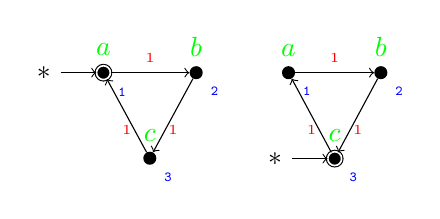
\begin{tikzpicture}[align=center,node distance=1cm]

    \vertex{above }{$\color{green}a$}{b2}{initial,accepting,state,scale=0.4}{below right}{1}
    \vertex{above }{$\color{green}b$}{b}{right =of b2}{below right}{2}
    \vertex{above }{$\color{green}c$}{b3}{below = of $(b2)!0.5!(b)$}{below right}{3}
    
        \vertex{above }{$\color{green}a$}{a2}{right = of b}{below right}{1}
    \vertex{above }{$\color{green}b$}{a}{right =of a2}{below right}{2}
    \vertex{above }{$\color{green}c$}{a3}{below = of $(a2)!0.5!(a)$, initial,accepting,state,scale=0.4}{below right}{3}
    
    
    \myedge{b2}{above}{$\scriptscriptstyle{\color{red}1}$}{b}
    \myedge{b}{below}{$\scriptscriptstyle{\color{red}1}$}{b3}
    \myedge{b3}{below}{$\scriptscriptstyle{\color{red}1}$}{b2}
    
    
    \myedge{a2}{above}{$\scriptscriptstyle{\color{red}1}$}{a}
    \myedge{a}{below}{$\scriptscriptstyle{\color{red}1}$}{a3}
    \myedge{a3}{below}{$\scriptscriptstyle{\color{red}1}$}{a2}
\end{tikzpicture}

\end{document}
